\newpage
\chapter{}
\section{Einleitung}
Das amtliche Höhensystem in Deutschland basiert auf Normalhöhen $H_N$. Bezugsfläche dieses Höhensystems ist das Quasigeoid. In dieser Übung sind 30 Festpunkten mit Ellipsoidische Höhen gegeben, 20 davon haben bekannte Normalhöhen. Die übrige Normalhöhen sind angefragt. 
\newpage

\section{Aufgabe}
\subsection{a}
Höhenanomalie
\begin{equation*}
	\zeta = h - H_N
\end{equation*}
wobei
\begin{itemize}
	\item $h$: ellpsoidische Höhe
	\item $H_N$: Normalhöhe
\end{itemize}
Höhenanomalie von Punkten 1 bis 20: 
\begin{table}[ht] \centering
	\begin{tabular}{|l|l|}
		\hline
		Pkt.Nr & Höhenanomalie [\ut{m}] \\ \hline
		1     & 48,3548       \\ \hline
		2     & 48,3928       \\ \hline
		3     & 48,4118       \\ \hline
		4     & 48,4159       \\ \hline
		5     & 48,4290       \\ \hline
		6     & 48,3750       \\ \hline
		7     & 48,4098       \\ \hline
		8     & 48,4360       \\ \hline
		9     & 48,4360       \\ \hline
		10    & 48,4487       \\ \hline
	\end{tabular}
	\begin{tabular}{|l|l|}
		\hline
		Pkt.Nr & Höhenanomalie [\ut{m}] \\ \hline
		11    & 48,3946       \\ \hline
		12    & 48,4203       \\ \hline
		13    & 48,4420      \\ \hline
		14    & 48,4556       \\ \hline
		15    & 48,4695      \\ \hline
		16    & 48,4148       \\ \hline
		17    & 48,4483       \\ \hline
		18    & 48,4659       \\ \hline
		19    & 48,4762       \\ \hline
		20    & 48,4890       \\ \hline
	\end{tabular}
\end{table}
\\
Standardabweichung
\begin{equation*}
	\sigma_{\zeta} = \sqrt{(\sigma_h^2 + \sigma_{H_N}^2)} = 0,0051 \ut{m}
\end{equation*}
Graphische Darstellung:
\begin{figure*}[ht]\centering
	\begin{subfigure}{.8\textwidth}
		\centering
		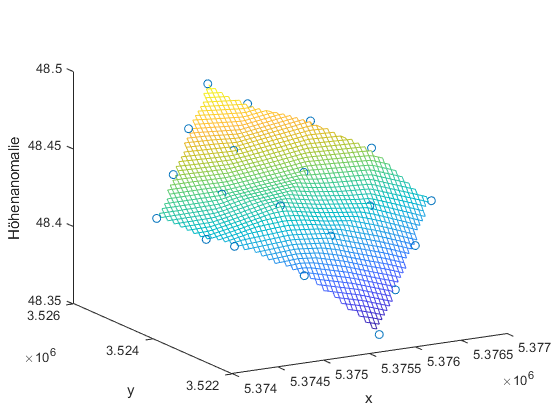
\includegraphics[width=.8\linewidth]{Images/Hoeheanomalie}  
		\caption{Höhenanomalie}
		\label{fig:sub-first}
	\end{subfigure}
\end{figure*}

\newpage
\subsection{b}
Der funktionale Modell:
\begin{gather*}
	\zeta_i = a_0 + a_1 \cdot y_i + a_2 \cdot x_i + a_3 \cdot y_i \cdot x_i + a_4 \cdot y_i^2 + a_5 \cdot x_i^2 \\
	\underbrace{\begin{bmatrix}
		\zeta_1 \\
		\zeta_2 \\
		\vdots \\
		\zeta_{19} \\
		\zeta_{20}
	\end{bmatrix}}_{\text{$l$}} = \underbrace{\begin{bmatrix}
		1 & y_1 & x_1 & y_1 \cdot x_1 & y_1^2 & x_1^2 \\
		1 & y_2 & x_2 & y_2 \cdot x_2 & y_2^2 & x_2^2 \\
		\vdots \\
		1 & y_{19} & x_{19} & y_{19} \cdot x_{19} & y_{19}^2 & x_{19}^2 \\
		1 & y_{20} & x_{20} & y_{20} \cdot x_{20} & y_{20}^2 & x_{20}^2 \\
	\end{bmatrix}}_{\text{$A$}} \cdot \underbrace{\begin{bmatrix}
		a_0 \\
		a_1 \\
		a_2 \\
		a_3 \\
		a_4 \\
		a_5
	\end{bmatrix}}_{\text{$x$}} \\
	\hat{x} = (A'A)^{-1}A'l = \begin{bmatrix}
		64990,1304 \\
		-0,0500 \\
		0,0086 \\
		1,3003 \cdot 10^{-8} \\
		-2,8173 \cdot 10^{-9} \\
		-5,0615 \cdot 10^{-9} \\
	\end{bmatrix}
\end{gather*}
\subsection{c}
$n$ ist die Anzahl der übrigen Koeffizienten, Redudanz $r = 20 - n$
\begin{gather*}
	\hat{\zeta} = A \cdot \hat{x} \\
	\hat{\varepsilon} = \zeta - \hat{\zeta} \\
	\sigma_{\hat{\zeta}} = \frac{\hat{\varepsilon}'\hat{\varepsilon}}{r} \\
	\sigma_a = \sigma_{\hat{\zeta}} \cdot (A'A)^{-1}
\end{gather*}
